% Options for packages loaded elsewhere
\PassOptionsToPackage{unicode}{hyperref}
\PassOptionsToPackage{hyphens}{url}
%
\documentclass[
]{article}
\title{MA7007 - Statistical Modelling and Forecasting Case Study Report
2023-2024}
\author{}
\date{\vspace{-2.5em}}

\usepackage{amsmath,amssymb}
\usepackage{lmodern}
\usepackage{iftex}
\ifPDFTeX
  \usepackage[T1]{fontenc}
  \usepackage[utf8]{inputenc}
  \usepackage{textcomp} % provide euro and other symbols
\else % if luatex or xetex
  \usepackage{unicode-math}
  \defaultfontfeatures{Scale=MatchLowercase}
  \defaultfontfeatures[\rmfamily]{Ligatures=TeX,Scale=1}
\fi
% Use upquote if available, for straight quotes in verbatim environments
\IfFileExists{upquote.sty}{\usepackage{upquote}}{}
\IfFileExists{microtype.sty}{% use microtype if available
  \usepackage[]{microtype}
  \UseMicrotypeSet[protrusion]{basicmath} % disable protrusion for tt fonts
}{}
\makeatletter
\@ifundefined{KOMAClassName}{% if non-KOMA class
  \IfFileExists{parskip.sty}{%
    \usepackage{parskip}
  }{% else
    \setlength{\parindent}{0pt}
    \setlength{\parskip}{6pt plus 2pt minus 1pt}}
}{% if KOMA class
  \KOMAoptions{parskip=half}}
\makeatother
\usepackage{xcolor}
\IfFileExists{xurl.sty}{\usepackage{xurl}}{} % add URL line breaks if available
\IfFileExists{bookmark.sty}{\usepackage{bookmark}}{\usepackage{hyperref}}
\hypersetup{
  pdftitle={MA7007 - Statistical Modelling and Forecasting Case Study Report 2023-2024},
  hidelinks,
  pdfcreator={LaTeX via pandoc}}
\urlstyle{same} % disable monospaced font for URLs
\usepackage[margin=1in]{geometry}
\usepackage{color}
\usepackage{fancyvrb}
\newcommand{\VerbBar}{|}
\newcommand{\VERB}{\Verb[commandchars=\\\{\}]}
\DefineVerbatimEnvironment{Highlighting}{Verbatim}{commandchars=\\\{\}}
% Add ',fontsize=\small' for more characters per line
\usepackage{framed}
\definecolor{shadecolor}{RGB}{248,248,248}
\newenvironment{Shaded}{\begin{snugshade}}{\end{snugshade}}
\newcommand{\AlertTok}[1]{\textcolor[rgb]{0.94,0.16,0.16}{#1}}
\newcommand{\AnnotationTok}[1]{\textcolor[rgb]{0.56,0.35,0.01}{\textbf{\textit{#1}}}}
\newcommand{\AttributeTok}[1]{\textcolor[rgb]{0.77,0.63,0.00}{#1}}
\newcommand{\BaseNTok}[1]{\textcolor[rgb]{0.00,0.00,0.81}{#1}}
\newcommand{\BuiltInTok}[1]{#1}
\newcommand{\CharTok}[1]{\textcolor[rgb]{0.31,0.60,0.02}{#1}}
\newcommand{\CommentTok}[1]{\textcolor[rgb]{0.56,0.35,0.01}{\textit{#1}}}
\newcommand{\CommentVarTok}[1]{\textcolor[rgb]{0.56,0.35,0.01}{\textbf{\textit{#1}}}}
\newcommand{\ConstantTok}[1]{\textcolor[rgb]{0.00,0.00,0.00}{#1}}
\newcommand{\ControlFlowTok}[1]{\textcolor[rgb]{0.13,0.29,0.53}{\textbf{#1}}}
\newcommand{\DataTypeTok}[1]{\textcolor[rgb]{0.13,0.29,0.53}{#1}}
\newcommand{\DecValTok}[1]{\textcolor[rgb]{0.00,0.00,0.81}{#1}}
\newcommand{\DocumentationTok}[1]{\textcolor[rgb]{0.56,0.35,0.01}{\textbf{\textit{#1}}}}
\newcommand{\ErrorTok}[1]{\textcolor[rgb]{0.64,0.00,0.00}{\textbf{#1}}}
\newcommand{\ExtensionTok}[1]{#1}
\newcommand{\FloatTok}[1]{\textcolor[rgb]{0.00,0.00,0.81}{#1}}
\newcommand{\FunctionTok}[1]{\textcolor[rgb]{0.00,0.00,0.00}{#1}}
\newcommand{\ImportTok}[1]{#1}
\newcommand{\InformationTok}[1]{\textcolor[rgb]{0.56,0.35,0.01}{\textbf{\textit{#1}}}}
\newcommand{\KeywordTok}[1]{\textcolor[rgb]{0.13,0.29,0.53}{\textbf{#1}}}
\newcommand{\NormalTok}[1]{#1}
\newcommand{\OperatorTok}[1]{\textcolor[rgb]{0.81,0.36,0.00}{\textbf{#1}}}
\newcommand{\OtherTok}[1]{\textcolor[rgb]{0.56,0.35,0.01}{#1}}
\newcommand{\PreprocessorTok}[1]{\textcolor[rgb]{0.56,0.35,0.01}{\textit{#1}}}
\newcommand{\RegionMarkerTok}[1]{#1}
\newcommand{\SpecialCharTok}[1]{\textcolor[rgb]{0.00,0.00,0.00}{#1}}
\newcommand{\SpecialStringTok}[1]{\textcolor[rgb]{0.31,0.60,0.02}{#1}}
\newcommand{\StringTok}[1]{\textcolor[rgb]{0.31,0.60,0.02}{#1}}
\newcommand{\VariableTok}[1]{\textcolor[rgb]{0.00,0.00,0.00}{#1}}
\newcommand{\VerbatimStringTok}[1]{\textcolor[rgb]{0.31,0.60,0.02}{#1}}
\newcommand{\WarningTok}[1]{\textcolor[rgb]{0.56,0.35,0.01}{\textbf{\textit{#1}}}}
\usepackage{graphicx}
\makeatletter
\def\maxwidth{\ifdim\Gin@nat@width>\linewidth\linewidth\else\Gin@nat@width\fi}
\def\maxheight{\ifdim\Gin@nat@height>\textheight\textheight\else\Gin@nat@height\fi}
\makeatother
% Scale images if necessary, so that they will not overflow the page
% margins by default, and it is still possible to overwrite the defaults
% using explicit options in \includegraphics[width, height, ...]{}
\setkeys{Gin}{width=\maxwidth,height=\maxheight,keepaspectratio}
% Set default figure placement to htbp
\makeatletter
\def\fps@figure{htbp}
\makeatother
\setlength{\emergencystretch}{3em} % prevent overfull lines
\providecommand{\tightlist}{%
  \setlength{\itemsep}{0pt}\setlength{\parskip}{0pt}}
\setcounter{secnumdepth}{-\maxdimen} % remove section numbering
\ifLuaTeX
  \usepackage{selnolig}  % disable illegal ligatures
\fi

\begin{document}
\maketitle

First, let's load the data, subset it for the specific age group, and
plot the histogram to find a suitable value for \texttt{nbins}.

\begin{Shaded}
\begin{Highlighting}[]
\CommentTok{\# Load the packages}
\FunctionTok{library}\NormalTok{(ggplot2)}
\FunctionTok{library}\NormalTok{(gamlss)}
\end{Highlighting}
\end{Shaded}

\begin{verbatim}
## Loading required package: splines
\end{verbatim}

\begin{verbatim}
## Loading required package: gamlss.data
\end{verbatim}

\begin{verbatim}
## 
## Attaching package: 'gamlss.data'
\end{verbatim}

\begin{verbatim}
## The following object is masked from 'package:datasets':
## 
##     sleep
\end{verbatim}

\begin{verbatim}
## Loading required package: gamlss.dist
\end{verbatim}

\begin{verbatim}
## Loading required package: nlme
\end{verbatim}

\begin{verbatim}
## Loading required package: parallel
\end{verbatim}

\begin{verbatim}
##  **********   GAMLSS Version 5.4-20  **********
\end{verbatim}

\begin{verbatim}
## For more on GAMLSS look at https://www.gamlss.com/
\end{verbatim}

\begin{verbatim}
## Type gamlssNews() to see new features/changes/bug fixes.
\end{verbatim}

\begin{Shaded}
\begin{Highlighting}[]
\FunctionTok{library}\NormalTok{(gamlss.ggplots)}
\end{Highlighting}
\end{Shaded}

\begin{verbatim}
## Loading required package: gamlss.foreach
\end{verbatim}

\begin{verbatim}
## Loading required package: foreach
\end{verbatim}

\begin{verbatim}
## Loading required package: doParallel
\end{verbatim}

\begin{verbatim}
## Loading required package: iterators
\end{verbatim}

\begin{Shaded}
\begin{Highlighting}[]
\FunctionTok{library}\NormalTok{(gamlss.add)}
\end{Highlighting}
\end{Shaded}

\begin{verbatim}
## Loading required package: mgcv
\end{verbatim}

\begin{verbatim}
## This is mgcv 1.9-0. For overview type 'help("mgcv-package")'.
\end{verbatim}

\begin{verbatim}
## Loading required package: nnet
\end{verbatim}

\begin{verbatim}
## 
## Attaching package: 'nnet'
\end{verbatim}

\begin{verbatim}
## The following object is masked from 'package:mgcv':
## 
##     multinom
\end{verbatim}

\begin{verbatim}
## Loading required package: rpart
\end{verbatim}

\begin{Shaded}
\begin{Highlighting}[]
\FunctionTok{library}\NormalTok{(gamlss.data)}
\FunctionTok{library}\NormalTok{(MASS)}

\CommentTok{\# Load the dataset}
\FunctionTok{data}\NormalTok{(dbbmi)}
\FunctionTok{summary}\NormalTok{(dbbmi)}
\end{Highlighting}
\end{Shaded}

\begin{verbatim}
##       age              bmi       
##  Min.   : 0.030   Min.   :11.17  
##  1st Qu.: 1.863   1st Qu.:15.96  
##  Median :10.450   Median :17.45  
##  Mean   : 9.291   Mean   :18.03  
##  3rd Qu.:15.130   3rd Qu.:19.60  
##  Max.   :21.700   Max.   :35.42
\end{verbatim}

\begin{Shaded}
\begin{Highlighting}[]
\CommentTok{\# Subset for ages 15 to 16}
\NormalTok{old }\OtherTok{\textless{}{-}} \DecValTok{15}
\NormalTok{dbbmi\_15 }\OtherTok{\textless{}{-}} \FunctionTok{with}\NormalTok{(dbbmi, }\FunctionTok{subset}\NormalTok{(dbbmi, age }\SpecialCharTok{\textgreater{}}\NormalTok{ old }\SpecialCharTok{\&}\NormalTok{ age }\SpecialCharTok{\textless{}}\NormalTok{ old }\SpecialCharTok{+} \DecValTok{1}\NormalTok{))}
\NormalTok{bmi15 }\OtherTok{\textless{}{-}}\NormalTok{ dbbmi\_15}\SpecialCharTok{$}\NormalTok{bmi}
\FunctionTok{summary}\NormalTok{(bmi15)}
\end{Highlighting}
\end{Shaded}

\begin{verbatim}
##    Min. 1st Qu.  Median    Mean 3rd Qu.    Max. 
##   14.70   18.29   19.45   19.75   20.84   35.03
\end{verbatim}

\begin{Shaded}
\begin{Highlighting}[]
\CommentTok{\# Plot the histogram; adjust nbins as needed to make the histogram look good}
\NormalTok{binwith }\OtherTok{=} \FloatTok{0.5}
\NormalTok{nbins }\OtherTok{=} \FunctionTok{trunc}\NormalTok{(}\FunctionTok{max}\NormalTok{(bmi15) }\SpecialCharTok{{-}} \FunctionTok{min}\NormalTok{(bmi15)) }\SpecialCharTok{/}\NormalTok{ binwith}

\FunctionTok{truehist}\NormalTok{(bmi15, }\AttributeTok{nbins=}\NormalTok{nbins)}
\end{Highlighting}
\end{Shaded}

\includegraphics{assignment_q1_bmi_files/figure-latex/histograms-1.pdf}

\begin{Shaded}
\begin{Highlighting}[]
\FunctionTok{density}\NormalTok{(bmi15, }\AttributeTok{cut =} \DecValTok{0}\NormalTok{)}
\end{Highlighting}
\end{Shaded}

\begin{verbatim}
## 
## Call:
##  density.default(x = bmi15, cut = 0)
## 
## Data: bmi15 (403 obs.);  Bandwidth 'bw' = 0.515
## 
##        x               y            
##  Min.   :14.70   Min.   :4.300e-07  
##  1st Qu.:19.78   1st Qu.:6.803e-04  
##  Median :24.87   Median :1.193e-02  
##  Mean   :24.87   Mean   :4.900e-02  
##  3rd Qu.:29.95   3rd Qu.:8.370e-02  
##  Max.   :35.03   Max.   :2.127e-01
\end{verbatim}

\begin{Shaded}
\begin{Highlighting}[]
\NormalTok{gamlss.ggplots}\SpecialCharTok{:::}\FunctionTok{y\_hist}\NormalTok{(dbbmi\_15}\SpecialCharTok{$}\NormalTok{bmi,}
                        \AttributeTok{from=}\FunctionTok{floor}\NormalTok{(}\FunctionTok{min}\NormalTok{(bmi15)), }
                        \AttributeTok{to=}\FunctionTok{ceiling}\NormalTok{(}\FunctionTok{max}\NormalTok{(bmi15)),}
                        \AttributeTok{binwidth=}\NormalTok{binwith,}
                        \AttributeTok{title=}\StringTok{"Histogram of BMI for 15 year olds"}\NormalTok{)}
\end{Highlighting}
\end{Shaded}

\includegraphics{assignment_q1_bmi_files/figure-latex/histograms-2.pdf}
Next, we'll fit several parametric distributions to the data. Common
distributions for BMI data include the Normal, Log-Normal, and Gamma
distributions, among others. The \texttt{gamlss} package provides
functions to fit a wide range of distributions.

\begin{Shaded}
\begin{Highlighting}[]
\CommentTok{\# Sense check our thought on skew and kurtosis by plotting against the Normal distribution}
\FunctionTok{plot}\NormalTok{(}\FunctionTok{histDist}\NormalTok{(bmi, }\StringTok{"NO"}\NormalTok{, }\AttributeTok{density=}\ConstantTok{TRUE}\NormalTok{, }\AttributeTok{line.col=}\FunctionTok{c}\NormalTok{(}\DecValTok{1}\NormalTok{,}\DecValTok{1}\NormalTok{), }\AttributeTok{line.ty=}\FunctionTok{c}\NormalTok{(}\DecValTok{1}\NormalTok{,}\DecValTok{2}\NormalTok{), }\AttributeTok{nbins=}\NormalTok{nbins, }\AttributeTok{data=}\NormalTok{dbbmi\_15))}
\end{Highlighting}
\end{Shaded}

\includegraphics{assignment_q1_bmi_files/figure-latex/fitDist-1.pdf}
\includegraphics{assignment_q1_bmi_files/figure-latex/fitDist-2.pdf}

\begin{verbatim}
## ******************************************************************
##        Summary of the Quantile Residuals
##                            mean   =  -4.708981e-07 
##                        variance   =  1.00249 
##                coef. of skewness  =  1.510098 
##                coef. of kurtosis  =  8.975065 
## Filliben correlation coefficient  =  0.9573336 
## ******************************************************************
\end{verbatim}

The choice of distribution can be justified by comparing the Akaike
Information Criterion (AIC) values of the fitted models---the model with
the lowest AIC is typically preferred as it suggests a good fit with
relatively lower complexity.

\begin{Shaded}
\begin{Highlighting}[]
\CommentTok{\# No explanitory variable so we can use fitDist to get the best dist for continuous distributions}
\NormalTok{f1 }\OtherTok{\textless{}{-}} \FunctionTok{fitDist}\NormalTok{(bmi, }\AttributeTok{type=}\StringTok{\textquotesingle{}realAll\textquotesingle{}}\NormalTok{, }\AttributeTok{data=}\NormalTok{dbbmi\_15, }\AttributeTok{k=}\DecValTok{2}\NormalTok{)}
\end{Highlighting}
\end{Shaded}

\begin{verbatim}
##   |                                                                              |                                                                      |   0%  |                                                                              |=                                                                     |   2%  |                                                                              |===                                                                   |   4%  |                                                                              |====                                                                  |   6%  |                                                                              |=====                                                                 |   8%  |                                                                              |=======                                                               |  10%  |                                                                              |========                                                              |  12%  |                                                                              |==========                                                            |  14%  |                                                                              |===========                                                           |  16%  |                                                                              |============                                                          |  18%  |                                                                              |==============                                                        |  20%  |                                                                              |===============                                                       |  22%  |                                                                              |================                                                      |  24%  |                                                                              |==================                                                    |  25%  |                                                                              |===================                                                   |  27%  |                                                                              |=====================                                                 |  29%  |                                                                              |======================                                                |  31%  |                                                                              |=======================                                               |  33%  |                                                                              |=========================                                             |  35%  |                                                                              |==========================                                            |  37%  |                                                                              |===========================                                           |  39%  |                                                                              |=============================                                         |  41%  |                                                                              |==============================                                        |  43%  |                                                                              |================================                                      |  45%  |                                                                              |=================================                                     |  47%  |                                                                              |==================================                                    |  49%  |                                                                              |====================================                                  |  51%  |                                                                              |=====================================                                 |  53%  |                                                                              |======================================                                |  55%  |                                                                              |========================================                              |  57%  |                                                                              |=========================================                             |  59%  |                                                                              |===========================================                           |  61%  |                                                                              |============================================                          |  63%  |                                                                              |=============================================                         |  65%  |                                                                              |===============================================                       |  67%  |                                                                              |================================================                      |  69%  |                                                                              |=================================================                     |  71%  |                                                                              |===================================================                   |  73%  |                                                                              |====================================================                  |  75%  |                                                                              |======================================================                |  76%  |                                                                              |=======================================================               |  78%  |                                                                              |========================================================              |  80%  |                                                                              |==========================================================            |  82%  |                                                                              |===========================================================           |  84%  |                                                                              |============================================================          |  86%  |                                                                              |==============================================================        |  88%  |                                                                              |===============================================================       |  90%  |                                                                              |=================================================================     |  92%  |                                                                              |==================================================================    |  94%  |                                                                              |===================================================================   |  96%  |                                                                              |===================================================================== |  98%  |                                                                              |======================================================================| 100%
\end{verbatim}

\begin{Shaded}
\begin{Highlighting}[]
\NormalTok{f1}\SpecialCharTok{$}\NormalTok{fits[}\DecValTok{1}\SpecialCharTok{:}\DecValTok{8}\NormalTok{]}
\end{Highlighting}
\end{Shaded}

\begin{verbatim}
##   exGAUS    BCPEo     BCPE     BCTo      BCT      ST5    BCCGo     BCCG 
## 1729.537 1729.731 1729.731 1729.992 1729.992 1730.401 1730.663 1730.663
\end{verbatim}

\begin{Shaded}
\begin{Highlighting}[]
\CommentTok{\# Validate fitDist by looking at the AIC for different GAIC penalties}
\NormalTok{m0 }\OtherTok{\textless{}{-}} \FunctionTok{gamlss}\NormalTok{(bmi }\SpecialCharTok{\textasciitilde{}} \DecValTok{1}\NormalTok{, }\AttributeTok{family=}\NormalTok{NO, }\AttributeTok{data=}\NormalTok{dbbmi\_15)}
\end{Highlighting}
\end{Shaded}

\begin{verbatim}
## GAMLSS-RS iteration 1: Global Deviance = 1803.044 
## GAMLSS-RS iteration 2: Global Deviance = 1803.044
\end{verbatim}

\begin{Shaded}
\begin{Highlighting}[]
\NormalTok{c1 }\OtherTok{\textless{}{-}} \FunctionTok{chooseDist}\NormalTok{(m0, }\AttributeTok{type=}\StringTok{\textquotesingle{}realAll\textquotesingle{}}\NormalTok{, }\AttributeTok{data=}\NormalTok{dbbmi\_15, }\AttributeTok{parallel=}\StringTok{"snow"}\NormalTok{, }\AttributeTok{ncpus=}\DecValTok{4}\NormalTok{)}
\end{Highlighting}
\end{Shaded}

\begin{verbatim}
## minimum GAIC(k= 2 ) family: exGAUS 
## minimum GAIC(k= 3.84 ) family: exGAUS 
## minimum GAIC(k= 6 ) family: exGAUS
\end{verbatim}

\begin{Shaded}
\begin{Highlighting}[]
\NormalTok{c1}
\end{Highlighting}
\end{Shaded}

\begin{verbatim}
##                 2     3.84        6
## NO       1807.044 1810.724 1815.044
## GU       2117.531 2121.211 2125.531
## RG       1733.816 1737.496 1741.816
## LO       1761.949 1765.629 1769.949
## NET      1759.479 1763.159 1767.479
## TF       1756.536 1762.056 1768.536
## TF2      1756.537 1762.057 1768.537
## PE       1766.779 1772.299 1778.779
## PE2      1766.783 1772.303 1778.783
## SN1      1809.044 1814.564 1821.044
## SN2      1755.128 1760.648 1767.128
## exGAUS   1729.537 1735.057 1741.537
## SHASH    1735.278 1742.638 1751.278
## SHASHo   1740.368 1747.728 1756.368
## SHASHo2  1740.098 1747.458 1756.098
## EGB2     1734.237 1741.597 1750.237
## JSU      1731.709 1739.069 1747.709
## JSUo     1739.039 1746.399 1755.039
## SEP1     1742.582 1749.942 1758.582
## SEP2     1749.584 1756.944 1765.584
## SEP3     1742.365 1749.725 1758.365
## SEP4     1732.778 1740.138 1748.778
## ST1      1734.015 1741.375 1750.015
## ST2      1737.021 1744.381 1753.021
## ST3      1735.795 1743.155 1751.795
## ST4      1733.081 1740.441 1749.081
## ST5      1732.808 1740.168 1748.808
## SST      1735.770 1743.130 1751.770
## GT       1757.541 1764.901 1773.541
## EXP      3212.376 3214.216 3216.376
## GA       1772.064 1775.744 1780.064
## IG       1759.441 1763.121 1767.441
## LOGNO    1758.605 1762.285 1766.605
## LOGNO2   1758.605 1762.285 1766.605
## WEI      1966.621 1970.301 1974.621
## WEI2     2373.622 2377.302 2381.622
## WEI3     1966.621 1970.301 1974.621
## IGAMMA   1748.193 1751.873 1756.193
## PARETO2  3251.903 3255.583 3259.903
## PARETO2o 3222.313 3225.993 3230.313
## GP       3251.903 3255.583 3259.903
## BCCG     1730.663 1736.183 1742.663
## BCCGo    1730.663 1736.183 1742.663
## GG       1732.317 1737.837 1744.317
## GIG      1750.193 1755.713 1762.193
## LNO      1758.605 1762.285 1766.605
## BCTo     1729.992 1737.352 1745.992
## BCT      1729.992 1737.352 1745.992
## BCPEo    1729.731 1737.091 1745.731
## BCPE     1729.731 1737.091 1745.731
## GB2      1732.204 1739.564 1748.204
\end{verbatim}

\begin{Shaded}
\begin{Highlighting}[]
\CommentTok{\# Here is out selected fitted distribution }
\NormalTok{fit\_exgaus }\OtherTok{\textless{}{-}} \FunctionTok{update}\NormalTok{(m0, }\AttributeTok{family=}\StringTok{"exGAUS"}\NormalTok{, }\AttributeTok{k=}\DecValTok{2}\NormalTok{)}
\end{Highlighting}
\end{Shaded}

\begin{verbatim}
## GAMLSS-RS iteration 1: Global Deviance = 1765.469 
## GAMLSS-RS iteration 2: Global Deviance = 1747.121 
## GAMLSS-RS iteration 3: Global Deviance = 1736.085 
## GAMLSS-RS iteration 4: Global Deviance = 1729.762 
## GAMLSS-RS iteration 5: Global Deviance = 1726.462 
## GAMLSS-RS iteration 6: Global Deviance = 1724.861 
## GAMLSS-RS iteration 7: Global Deviance = 1724.121 
## GAMLSS-RS iteration 8: Global Deviance = 1723.791 
## GAMLSS-RS iteration 9: Global Deviance = 1723.647 
## GAMLSS-RS iteration 10: Global Deviance = 1723.584 
## GAMLSS-RS iteration 11: Global Deviance = 1723.557 
## GAMLSS-RS iteration 12: Global Deviance = 1723.546 
## GAMLSS-RS iteration 13: Global Deviance = 1723.541 
## GAMLSS-RS iteration 14: Global Deviance = 1723.538 
## GAMLSS-RS iteration 15: Global Deviance = 1723.537
\end{verbatim}

The Best fit is exGAUS

\begin{Shaded}
\begin{Highlighting}[]
\CommentTok{\# Plot out the distribution with the lowest GAIC}
\NormalTok{m\_exgaus }\OtherTok{\textless{}{-}} \FunctionTok{histDist}\NormalTok{(bmi, }\StringTok{"exGAUS"}\NormalTok{, }\AttributeTok{density=}\ConstantTok{TRUE}\NormalTok{, }\AttributeTok{line.col=}\FunctionTok{c}\NormalTok{(}\DecValTok{1}\NormalTok{,}\DecValTok{1}\NormalTok{), }\AttributeTok{line.ty=}\FunctionTok{c}\NormalTok{(}\DecValTok{1}\NormalTok{,}\DecValTok{2}\NormalTok{), }\AttributeTok{nbins=}\NormalTok{nbins, }\AttributeTok{data=}\NormalTok{dbbmi\_15)}
\end{Highlighting}
\end{Shaded}

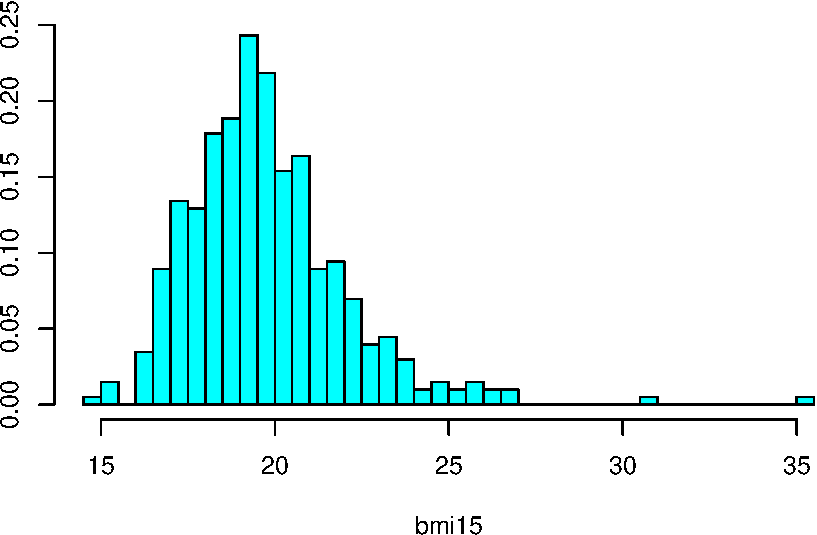
\includegraphics{assignment_q1_bmi_files/figure-latex/unnamed-chunk-1-1.pdf}

\begin{Shaded}
\begin{Highlighting}[]
\FunctionTok{plot}\NormalTok{(fit\_exgaus)}
\end{Highlighting}
\end{Shaded}

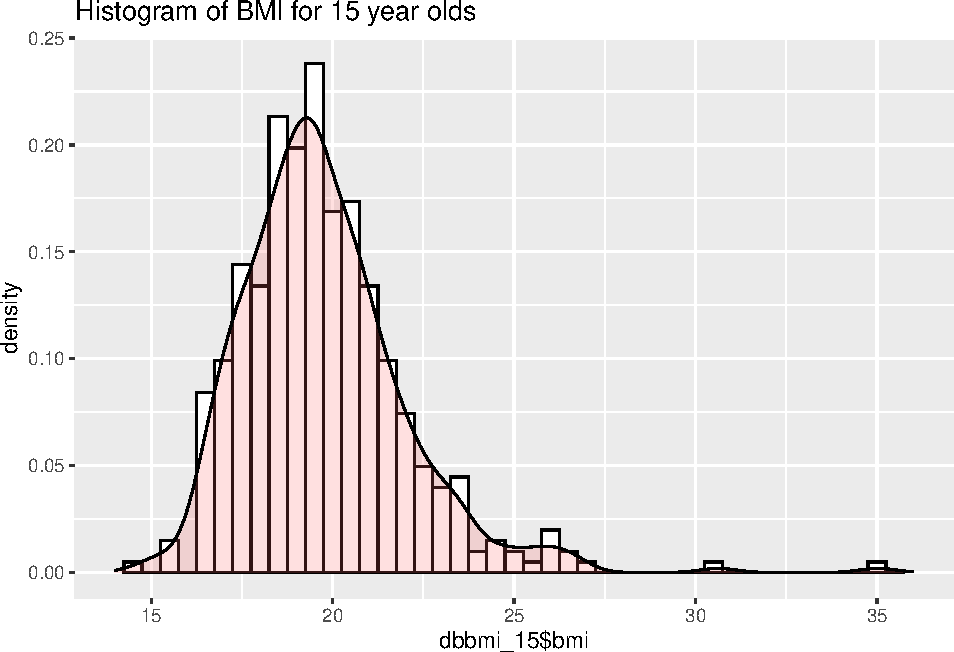
\includegraphics{assignment_q1_bmi_files/figure-latex/unnamed-chunk-1-2.pdf}

\begin{verbatim}
## ******************************************************************
##        Summary of the Quantile Residuals
##                            mean   =  -0.002651679 
##                        variance   =  1.00657 
##                coef. of skewness  =  0.06159507 
##                coef. of kurtosis  =  3.194194 
## Filliben correlation coefficient  =  0.9982055 
## ******************************************************************
\end{verbatim}

\begin{Shaded}
\begin{Highlighting}[]
\FunctionTok{wp}\NormalTok{(fit\_exgaus)}
\end{Highlighting}
\end{Shaded}

\includegraphics{assignment_q1_bmi_files/figure-latex/unnamed-chunk-1-3.pdf}

Finally, for the chosen model, we can output the parameter estimates and
interpret them according to the distribution's characteristics.

\begin{Shaded}
\begin{Highlighting}[]
\CommentTok{\# Value of fitted parameters}
\FunctionTok{fitted}\NormalTok{(f1, }\StringTok{"mu"}\NormalTok{)[}\DecValTok{1}\NormalTok{]}
\end{Highlighting}
\end{Shaded}

\begin{verbatim}
## [1] 17.94824
\end{verbatim}

\begin{Shaded}
\begin{Highlighting}[]
\FunctionTok{fitted}\NormalTok{(f1, }\StringTok{"sigma"}\NormalTok{)[}\DecValTok{1}\NormalTok{]}
\end{Highlighting}
\end{Shaded}

\begin{verbatim}
## [1] 1.277047
\end{verbatim}

\begin{Shaded}
\begin{Highlighting}[]
\FunctionTok{fitted}\NormalTok{(f1, }\StringTok{"nu"}\NormalTok{)[}\DecValTok{1}\NormalTok{]}
\end{Highlighting}
\end{Shaded}

\begin{verbatim}
## [1] 1.800627
\end{verbatim}

\begin{Shaded}
\begin{Highlighting}[]
\CommentTok{\# Output parameter estimates for the chosen model}
\FunctionTok{summary}\NormalTok{(fit\_exgaus)}
\end{Highlighting}
\end{Shaded}

\begin{verbatim}
## ******************************************************************
## Family:  c("exGAUS", "ex-Gaussian") 
## 
## Call:  gamlss(formula = bmi ~ 1, family = "exGAUS", data = dbbmi_15,  
##     k = 2) 
## 
## Fitting method: RS() 
## 
## ------------------------------------------------------------------
## Mu link function:  identity
## Mu Coefficients:
##             Estimate Std. Error t value Pr(>|t|)    
## (Intercept)  17.9521     0.1492   120.3   <2e-16 ***
## ---
## Signif. codes:  0 '***' 0.001 '**' 0.01 '*' 0.05 '.' 0.1 ' ' 1
## 
## ------------------------------------------------------------------
## Sigma link function:  log
## Sigma Coefficients:
##             Estimate Std. Error t value Pr(>|t|)   
## (Intercept)  0.24593    0.08047   3.056  0.00239 **
## ---
## Signif. codes:  0 '***' 0.001 '**' 0.01 '*' 0.05 '.' 0.1 ' ' 1
## 
## ------------------------------------------------------------------
## Nu link function:  log 
## Nu Coefficients:
##             Estimate Std. Error t value Pr(>|t|)    
## (Intercept)  0.58625    0.09008   6.508 2.28e-10 ***
## ---
## Signif. codes:  0 '***' 0.001 '**' 0.01 '*' 0.05 '.' 0.1 ' ' 1
## 
## ------------------------------------------------------------------
## No. of observations in the fit:  403 
## Degrees of Freedom for the fit:  3
##       Residual Deg. of Freedom:  400 
##                       at cycle:  15 
##  
## Global Deviance:     1723.537 
##             AIC:     1729.537 
##             SBC:     1741.534 
## ******************************************************************
\end{verbatim}

Interpretation of the parameters will depend on the selected
distribution.

\end{document}
